\documentclass[a4paper,11pt]{article}
\usepackage[latin1]{inputenc}
\usepackage[T1]{fontenc}
\usepackage{amsmath}
\usepackage{a4wide}
\usepackage{booktabs}
\usepackage{color}
\usepackage{soul} % highlighting

\usepackage{graphicx}
\usepackage[center,footnotesize]{caption}
\usepackage[section]{placeins}
%\usepackage{subfig}
\usepackage{subcaption}
\usepackage{wrapfig}

\title{Genomics and Bioinformatics}
\date{November 1, 2011}
\author{Examination - Week 7}
\begin{document}


\section*{Question 3}
\begin{enumerate}

\item Let us call T a transmembrane domain, E an extracellular domain, I an intracelular domain. 
Then the hidden states are T, E and I.
The model generates sequences of amino-acids which are the observations. 
The emission and transition matrices are defined in the following points.

One can either use two identical states T, in order to prevent transitions of the type E$\rightarrow$ T$\rightarrow$ E, 
or a single one between E and I.

\begin{figure}[hbt]
\centering
\begin{subfigure}[b]{0.3\textwidth}
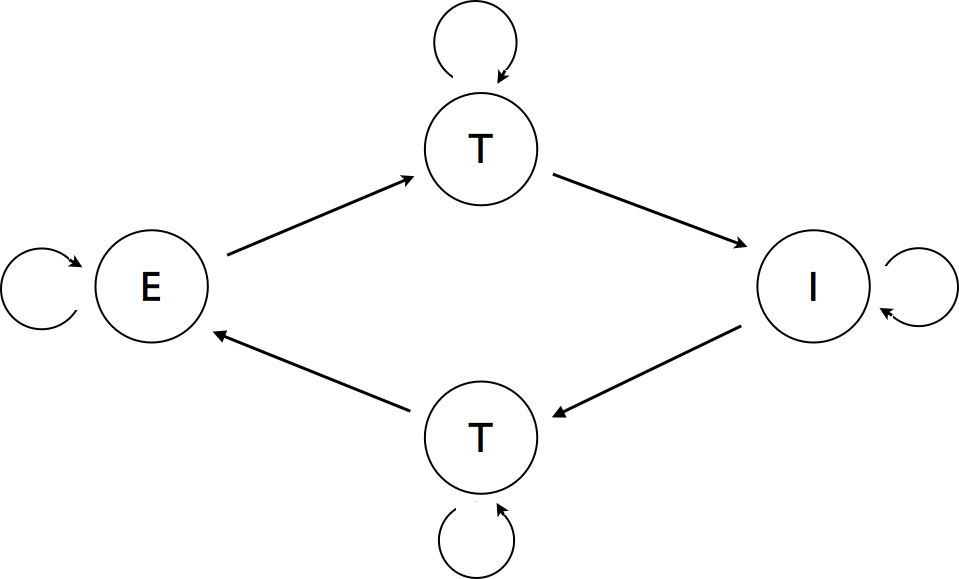
\includegraphics[width=\textwidth]{figures/hmm_graph1.png}
\caption{With two ``T'' states}
\end{subfigure}
\qquad
\begin{subfigure}[b]{0.3\textwidth}
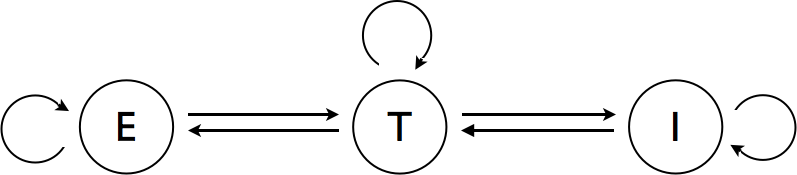
\includegraphics[width=\textwidth]{figures/hmm_graph2.png}
\\\\
\caption{With one ``T'' state}
\end{subfigure}
\end{figure}

There may be other possible models, but we give the solution only for these two.

\item The emissions from the T state are given by the helical propensity table, since we defined transmembrane domains as 
helices, and helices contain amino-acids with these fractions. In other domains, since all amino-acids are equiprobable and there
are 20 of them, each of them has a $1/20$ = $5\%$ frequency.

\item As we saw in an earlier exercise, the transition probabilities can be set as the inverse of the segment length.
In this case, there are about 20 amino-acids in a transmembrane domain, so one can set the probability of
going out of T as $1/20$. 

If we use two T states (a), both T $\rightarrow$ E and T $\rightarrow$ I transitions have to 
be set to $1/20$.

If you use a single T state (b), the sum of outgoing probabilities from T has to be $1/20$ - the easiest
is to choose $1/40$ for both T $\rightarrow$ E and T $\rightarrow$ I. 
All outgoing probabilities must sum to 1, so the transition T $\rightarrow$ T is $19/20$. 

For the E state, the outgoing probability is $1/500$ and the transition E $\rightarrow$ E is the complement 
$499/500$. For I we have $1/200$ and $199/200$. Finally, we obtain the following transition matrix:
$$
\begin{array}{c}
E \\ T_1 \\ I \\ T_2
\end{array}
\left( 
\begin{array}{cccc}
499/500 & 1/500 & 0            & 0 \\
0            & 19/20 & 1/20       & 0 \\
0            & 0        & 199/200 & 1/200 \\
1/20       & 0        & 0            & 19/20 \\
\end{array}
\right)
\quad or \quad 
\begin{array}{c}
E \\ T \\ I
\end{array}
\left( 
\begin{array}{ccc}
499/500 & 1/500 & 0 \\
1/40       & 19/20 & 1/40 \\
0            & 1/200 & 199/200 
\end{array}
\right)
$$

\item One can use either the Forward or Backward algorithm.

\item If $O_n$ is the n-th observation and $S_n$ is the state producing $O_n$, one can write 
$$P(O|S) = P(O_1O_2O_3... | S_1S_2S_3...) = P(O_1|S_1)\cdot P(O_2|S_2)\cdot P(O_3|S_3)\cdot ...$$
Since emissions are equally probable in states E and I, we can consider them equal in the calculation.
For our sequence, we have $P(O_1|S_1) = P(N|E) = 5\%$, $P(O_2|S_2) = P(G|E) = 5\%$, $P(O_3|S_3) = P(A|T) = 8\%$, etc.,
which gives in the end
$$P(O|S) = (5\cdot 5\cdot 8\cdot 6\cdot 5\cdot 5\cdot 5) / 100^{7} = 1.5\cdot 10^{5} / 10^{14} = 1.5\cdot 10^{-9}$$

\item If transmembrane domains always contain a multiple of 4 amino-acids, one can extend the model as follows, for instance:

\begin{figure}[hbt]
\centering
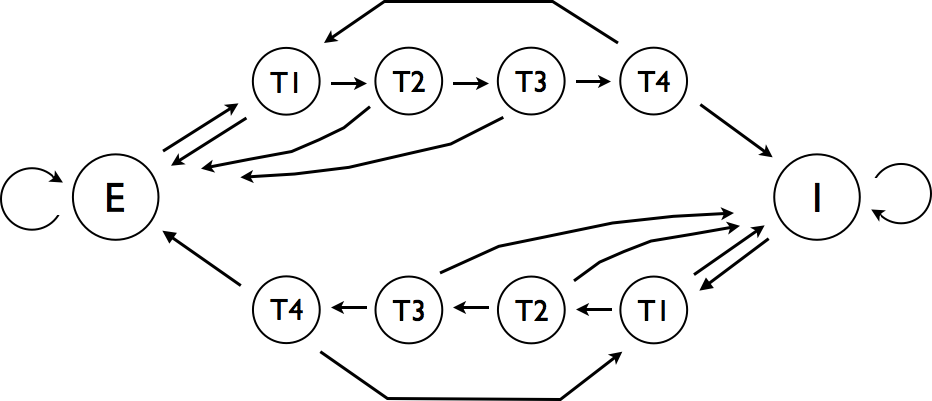
\includegraphics[width=0.6\textwidth]{figures/hmm_graph3.png}
\caption{A possible model. \\From the most probable sequence of states, the alpha-helices \\
are the domains with repeats of $T_1$ - $T_4$.}
\end{figure}


\end{enumerate}

\end{document}
